%----------------------------------------------------------------------------
\section{Az arclenyomatban kódolt személyes adatok vizsgálata} %(10-12 oldal)}
\label{sec:5}
%----------------------------------------------------------------------------

% \begin{itemize}
% 	\item elgondolás, ötlet, mire számítottunk
% 	\item Legfontosabb embedding feature-ök meghatározása (kutatási jelentésből) (4 oldal)
% 	\item Legfontosabb feature-ök eltávolítása, módosítása milyen hatással van a modell pontosságára (kutatási jelentésből) 
% 	\item Eredmények kiértékelése (kutatási jelentésből) 
% 	\item Arclenyomatvektor feature-einek köncsönös összefüggésének vizsgálata (diploma A-ból) (5 oldal)
% \end{itemize}

Az előző fejezetben bemutattam, hogy az arclenyomatokból jó pontossággal kinyerhetőek személyes adatok. A továbbiakban azza foglalkozom, hogy a személyes adatok hogyan vannak kódolva az arclenyomatokban, melyek azok a feature-ök amelyek alapján következtetni lehet az adatokra. Ehhez kiindulásnak vettem a betanított becslő modelleket, és azokon kísérleteztem.

Az elképzelésem az volt, hogy ha képesek vagyunk meghatározni az arclenyomatnak azon jellemzőit, amelyek például az illető rasszáról tartalmaz információt, akkor azon jellemzők módosításával elérhető lehet, hogy a módosított arclenyomatból ne lehessen következtetni az illető rasszára. Tehát valamilyen technikával maszkolná az információt. Ahhoz, hogy az arclenyomat a hassznosságából ne veszítsen, annak továbbra is használhatónak kell lennie az eredeti célra: az arcfelismerésre.

Első próbálkozásom az volt, hogy meghatározzam az arclenyomat azon jellemzőit amelyek a legtöbb információt tartalmazták, azaz azokat amelyek az osztályozó modell számára a legfontosabbak. Feltételezésem az volt, hogy ha módosítom az osztályozó modell számára legfontosabb jellemzők értékeit, akkor annak hatására jelentősen romlani fog a modell pontossági metrikát. így elérhető lehet az, hogy az érzékeny adat becslése pontatlan lesz, míg az identifikáció továbbra is jó pontossággal működik. Az elképzelés igazolásához az arclenyomatokat úgy próbáltam módosítani, hogy abból ne lehessen pontosan következtetni az képen látható személy rasszára. Ehhez szükségem volt meghatározni, hogy egy adott modellnek mely jellemzők járulnak leginkább hozzá a modell predikciójához.

\subsection{Top jellemzők meghatározása}

Ezek közül először a LIME \cite{lime2016} könyvtárat használtam, ami kifejezetten gépi tanulási modellek értelmezésére szolgál. A LIME könyvtár segítségével meg tudtuk határozni egy adott modell legfontosabb jellemzőit. A következő diagramon az egyes jellemzők előfordulási gyakoriságai láthatók. Például az (’f83’, 982) esetén az f83 jelöli az adott jellemzőt, az 982 pedig, hogy az 1000 LIME magyarázatból hányszor volt benne a 10 legfontosabb jellemző között. A 10 legfontosabb jellemzőt a \ref{fig:lime}. ábra mutatja.

\begin{figure}[ht]
	\centering
	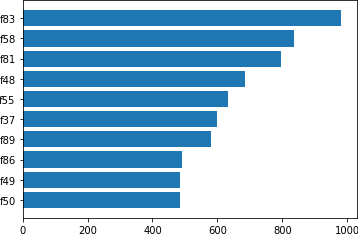
\includegraphics[width=0.7\columnwidth]{figures/imp_lime.png}
	\caption{Top 10 legfontosabb jellemző meghatározása LIME-mal.}
	\label{fig:lime}
\end{figure}

Annak érdekében, hogy az így kapott eredményeket megerősítsem, több, eltérő módszerrel is megvizsgáltam a modelleket. A Scikit-learn saját, modell-specifikus implementációját használtam. Ez a módszer kifejezetten döntési fa alapú modellekre alkalmazható. A döntési fákban magasabban található jellemzők nagyobb fontosságúak, mint az alacsonyabban találhatóak. A módszer a Mean Decrease in Impurity és a, Gini importance-en alapul \cite{breiman2017classification}.

\begin{figure}[ht]
	\centering
	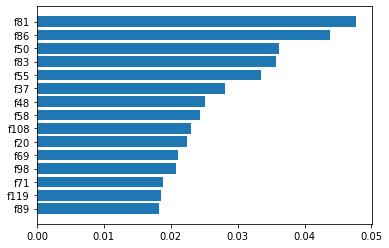
\includegraphics[width=0.7\columnwidth]{figures/imp_gini.png}
	\caption{Top 15 jellemző meghatározása a Scikit-learn módszerével.}
\end{figure}

A Permutation importance egy modellfüggetlen módszer. Én az eli5 \cite{eli5_2016} könyvtár implementációját használtam. Egy jellemző fontosságát meghatározhatjuk úgy, hogy megnézzük mennyivel csökken a modell pontossági metrikái (F1, $R^2$ stb.) ha egy adott jellemzőt eltávolítunk. Egy jellemző eltávolítása után újratanítjuk a modellt, és összehasonlítjuk a pontosságát az eredeti modell pontosságával. Mivel újratanítás szükséges, ez egy eléggé számításigényes eljárás.

\begin{figure}[ht]
	\centering
	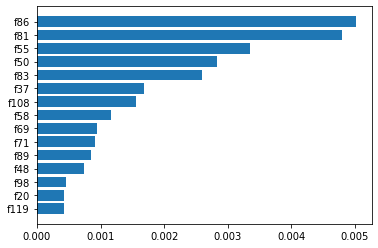
\includegraphics[width=0.7\columnwidth]{figures/imp_eli.png}
	\caption{Top 15 jellemző meghatározása permutation importance módszerrel.}
\end{figure}

Tree-SHAP \cite{treeshap2020} használatával elemezhetjük egy-egy megfigyelés esetén a jellemzők fontosságát, illetve globális összegző képet is kaphatunk egy adathalmazról. A Tree-SHAP kifejezetten döntési fa alapú modellekre optimalizált módszer, de használható Kernel SHAP is. Rassz predikció esetén halmozott oszlopdiagramon láthatjuk, hogy osztályonként (itt rasszonként) mely jellemzők a legjelentősebbek. Összegezve őket a korábbiakhoz hasonló eredményeket kapunk. A SHAP-pal kapott eredményta a \ref{fig:shap}. ábrán láthatjuk.

\begin{figure}[ht]
	\centering
	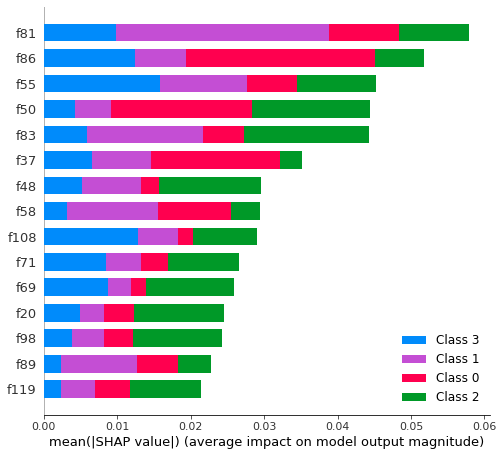
\includegraphics[width=0.7\columnwidth]{figures/imp_shap.png}
	\caption{Top 15 jellemző meghatározássa Tree-SHAP könyvtárral.}
	\label{fig:shap}
\end{figure}

Összegezve a négy módszerrel hasonló eredményeket kaptam. A legfontosabb jellemzők sorrendje csak kis mértékben tér el a módszerek között. Az egyes módszerek eredményeit összegeztem, majd az alapján létrehoztam egy fontossági listát az összes jellemzőről.

\subsection{Legfontosabb jellemzők kivétele.}

Miután meghatároztam a rassz osztályozó modell jellemzőinek fontossági sorrendjét, kipróbáltam, hogy a jellemzők eltávolítása milyen hatással van a modell pontosságára. Itt az elgondolás az volt, hogy ha a legfontosabb jellemzők közül 10-20-at eltávolítunk, azzal jelentősen lerontható a rassz modell pontossága. Nyilván ezt azt is jelentené, hogy az identifikációs modell pontossága is romlana valamennyire, viszont várhatóan kevésbé, mint a rassz predikciós modell pontossága. Az identifikációs modell az arclenyomatok alapján minden személyhez kiszámol egy centroidot, ami egy-egy pontként képzelhető el 128 dimenziós térben. A dimenziók csökkentésével a centroidok közelebb kerülnek egymáshoz, de amíg jól elkülönülnek egymástól, addig az identifikáció működhet.

Az elgondolás igazolásához írtam egy Python scriptet, ami az eredetileg $N \times 128$ dimenziójú tanító mintakészlet alapján betanítja a rassz osztályozó modellt, illetve az identifikációs modellt. Ez után iterációnként eltávolítja az 5 legfontosabbnak ítélt jellemzőt a mintákból, így az első iterációnál $N \times 123$ dimenziójú mintakészlet marad. A csökkentett dimenziójú mintákon majd egy új rassz osztályozó modelllt és identifikációs modellt tanítok be. Minden iterációban a teszt mintakészleten kiszámolom a modellek pontosságát. A jellemzők kivételét egészen addig folytatom, míg azok el nem fogynak. 

A mérés eredményeit a \ref{fig:retrain}. ábra mutatja be. Az x tengelyen a kivett jellemzők számát láthatjuk, az y tengelyen a modellek pontosságát. A narancs szaggatott vonal az identifikációs modell pontossága, a kék pontozott pedig a rassz predikciós modell pontossága. Számomra meglepő módon a modellek rendkívűl ellenállóak a jellemzők eltávolításával szemben. A 128 jellemzők felének eltávolításánál sem változott jelentősen a modellek pontossága. Az identifikáció modell egészen a piros függőleges vonalig ($x$ = 95, $y_{id}$ = 0.980, $y_{race}$ = 0.769) nem romlott jelentősen, majd utána meredeken letörik.

\begin{figure}[ht]
	\centering
	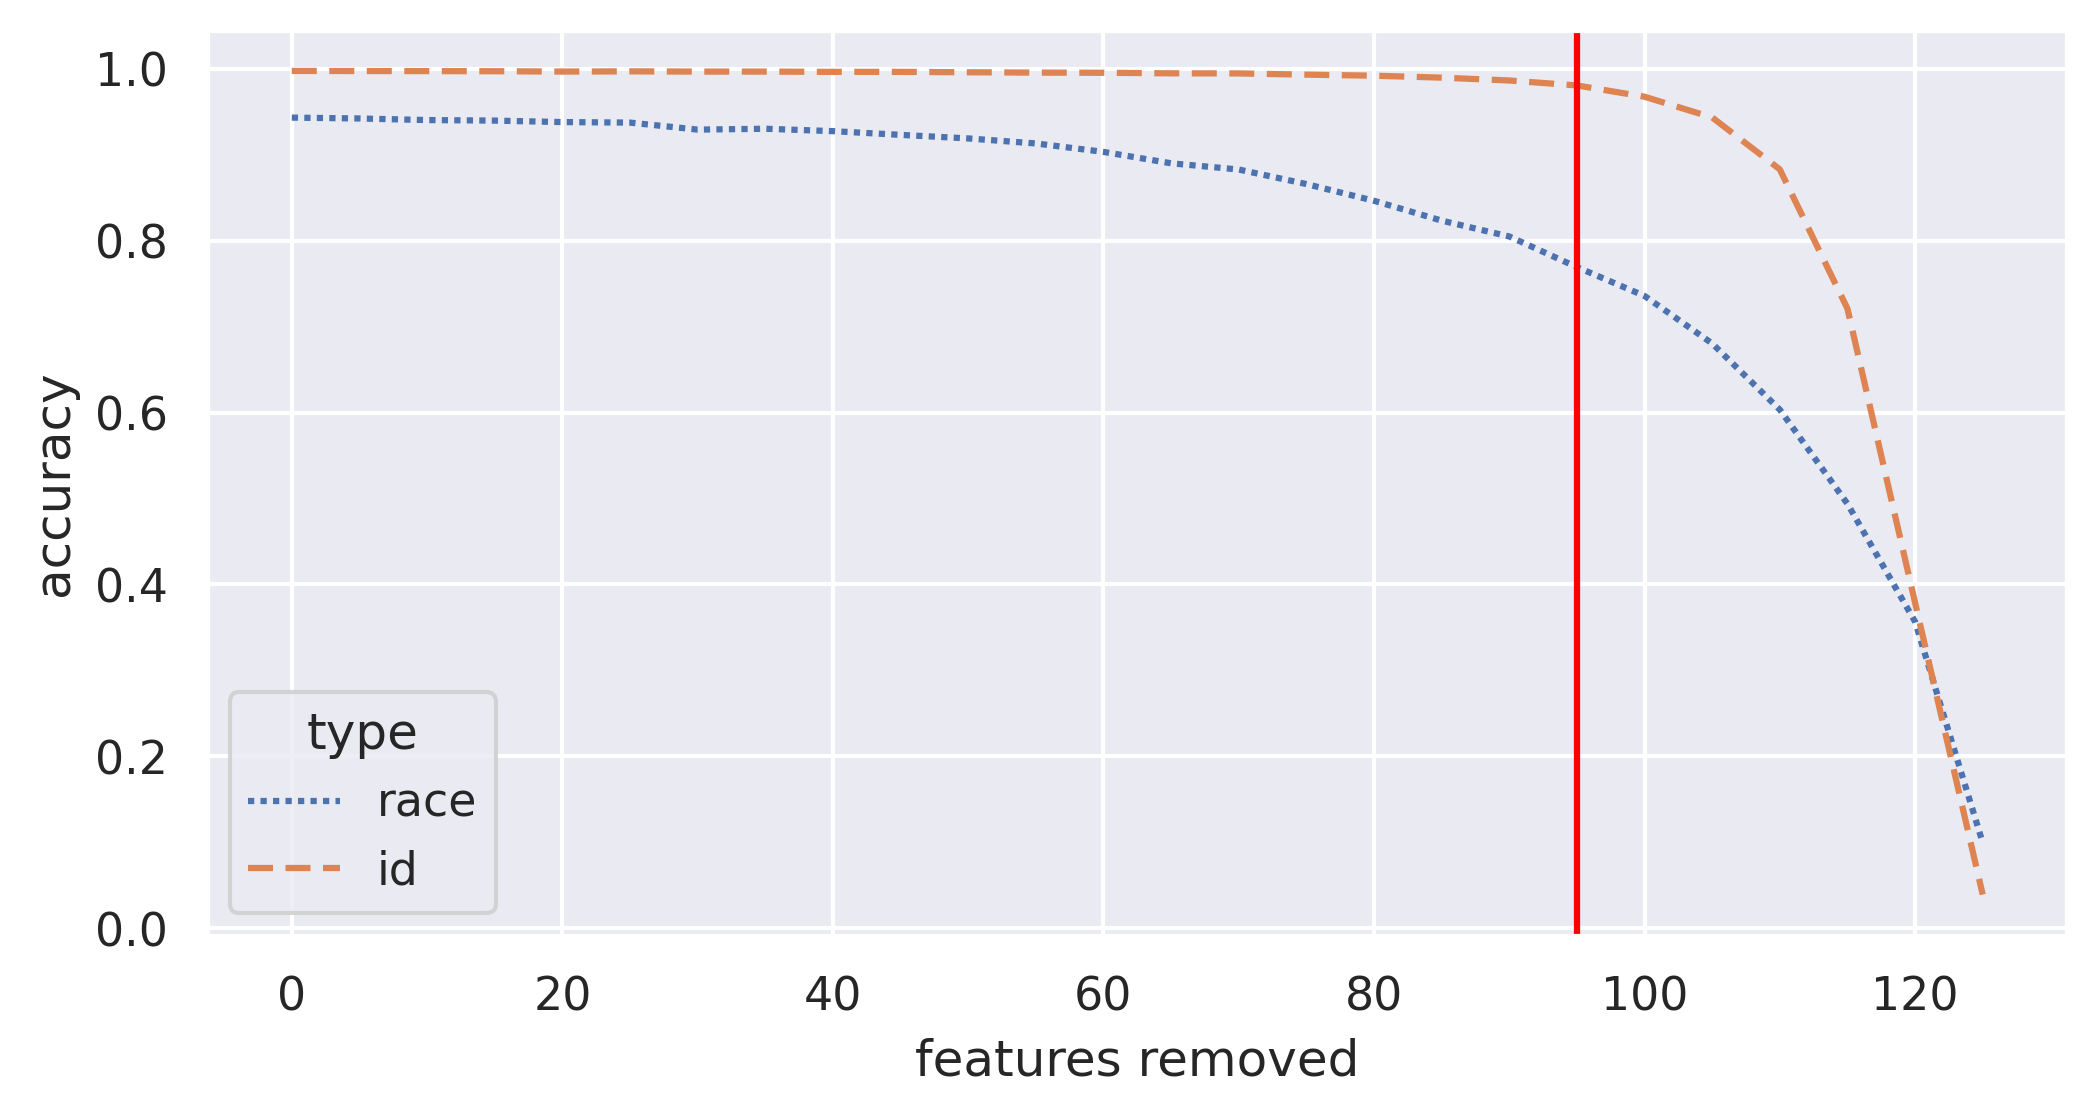
\includegraphics[width=0.9\columnwidth]{figures/imp_race_id_graph.png}
	\caption{szoveg}
	\label{fig:retrain}
\end{figure}

% conclusion?
A mérésből azt a következtetést vontam, hogy az egyes jellemzők eltávolítása nem elég az érzékeny adatok védelmére. Az tapasztaltam, hogy a modellek eléggé robusztusok, mivel nagyon sok jellemzőt (80-100) kell eltávolítani ahhoz, hogy a rassz osztályozó modell pontossága jelentősen romoljon. A korábbi módszerekkel kapott eredmények nem az elvártak szerint alakultak, ezért az egyes jellemzők összefüggőségét kezdtem vizsgálni. Ez a viselkedés az összetett hálózatoknál megfigyelt robusztusságra hasonlít \cite{albert2000error}. Azt feltételeztem, hogy a jellemzők értékei között kölcsönös függések állhatnak fent. A következő fejezetben a jellemzők közötti kölcsönös összefüggéseket vizsgálom.

% 
% We can conclude from these findings that removing individ- ual embedding features is not enough and counterproductive; we lose more utility than what we gain on the protection side. What is behind this robustness? The pattern resembles ro- bustness that we would expect from complex networks [4]. Simply put, if we remove nodes from such networks that adds damages to the overall connectivity, but links act as a backup for each other, and therefore we need to introduce damage to a large fraction to achieve notable results. In the next subsection we will investigate this issue.

% KUTATÁSI JELENTÉS
% -----------------------------------------------------------------------------

\subsection{Hálózat effektus vizsgálata}

Az arclenyomat vektorok korábbi vizsgálata kapcsán beláttuk, hogy a véletlen erdő (angol szakirodalomban random forest) modell döntési fáiban kölcsönös összefüggések állhatnak fent. Az volt a megfigyelésünk, hogy ez a kölcsönös összefüggés hasonlít ahhoz, amit komplex hálózatoknál tapasztalhatóak. Az ilyen hálózatoknál egy csomópont eltávolítása nincs nagy hatással a hálózatra, hanem több csomópont együttes kivételével lehet jelentősen rontani a hálózat összefüggőségén. 

Először megnéztem, hogy az arclenyomat vektorokon betanított véletlen erdő modellt át lehet-e transzformálni egy gráf reprezentációba. Miután ez sikerült, az volt a hipotézisünk, hogy a rassz predikciós modell és az arc identifikációs modellekből létrehozott gráfok együttes elemzésével találhatunk olyan csomópontokat, amelyek szignifikánsak a rassz predikciós gráfnál, viszont nem szignifikáns az identifikációs modell esetén. Így találhatunk módot az arclenyomat vektorokban hordozott érzékeny információk védelmére. 

\subsubsection*{Hálózat effektus vizsgálata Iris adathalmazon}
A véletlen erdő modell több döntési fát foglal magában. A vizsgálat során alap esetben 100 fából álló modellt alkalmaztam. Egy adott arclenyomat vektor bemenet esetén az erdőben található összes döntési fa képez egy szavazatot az egyik osztályra. Mivel az arclenyomat vektorokra betanított véletlen erdő rendkívül bonyolult döntési fákból áll, melyek működése ember számára már nem igazán értelmezhető, ezért kezdetben egy jelentősen kisebb adathalmazon: az Iris adathalmazon \cite{iris1936} végeztem a döntési fák vizsgálatát. Ez az adathalmaz négy jellemzőt (petal width (PW), petal length (PL), sepal width (SW), sepal length (SL) tartalmaz, és három kimeneti osztályt, ami három féle virágnak felel meg (setosa, versicolor, virginica). 

\begin{figure}[ht]
	\centering
	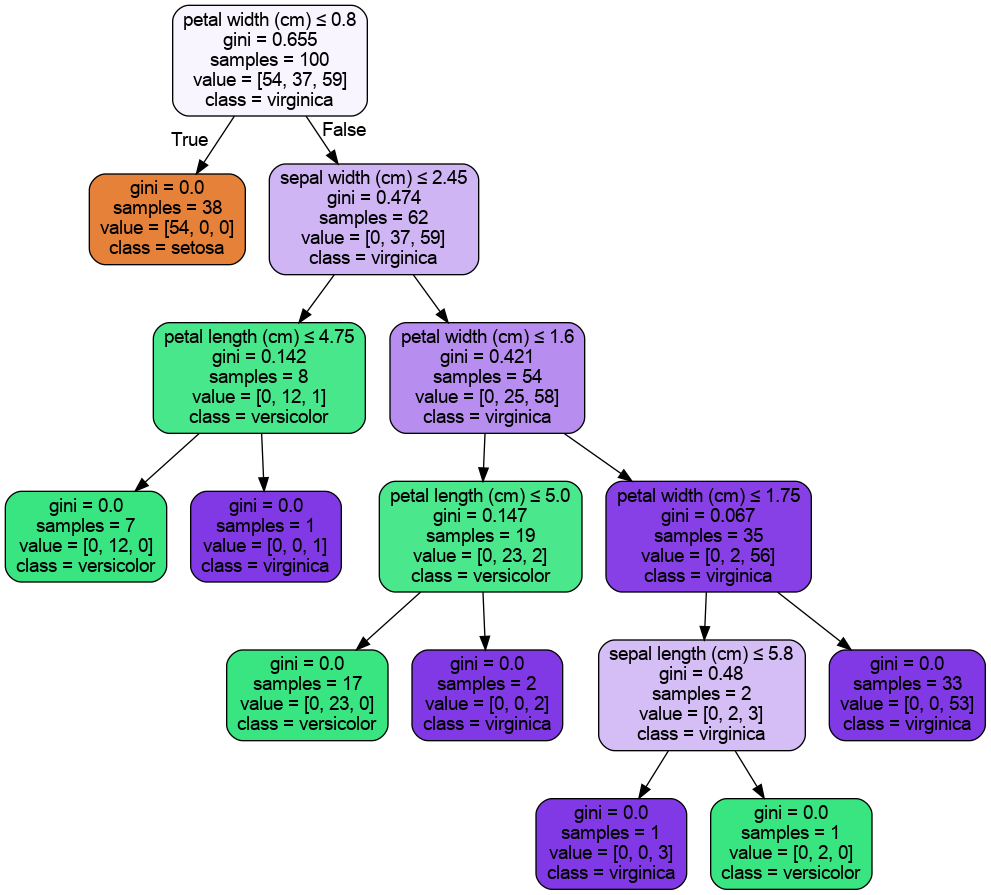
\includegraphics[width=0.9\columnwidth]{figures/network_iris_tree.png}
	\caption{Az Iris datasetre betanított véletlen erdő egyik döntési fája
	vizualizálva.}
\end{figure}

Az általam írt algoritmus célja a random forest classifiert átalakítani egy gráf reprezentációba. Az algoritmus először végighalad az erdőben lévő döntési fákon, és egy rekurzív függvény segítségével végig lép a döntési fa egyes csomópontjain. Egy adott csomópont lehet elágazás vagy levél. Elágazás esetén vizsgálni tudjuk az elágazás feltételét, ami egy adott jellemzőből, és egy küszöbértékből (threshold) áll. Az algoritmus működése során feltérképezi a teljes döntési fát, és kigyűjti az egyes levél csomópontokhoz tartozó feltétel rendszereket, azaz milyen feltételeknek kell teljesülnie ahhoz, hogy a döntési fa az adott levélre jusson. Feltételezésem az volt, hogy a fának azon feltételei lesznek szignifikánsak, amelyek gyakran fordulnak elő más feltételekkel együtt. Definiáltam egy NxN-es mátrixot, ahol N a jellemzők számát jelenti, és a mátrixot 0 értékekkel inicializáltam. A fa feltérképezése során a két jellemzőhöz kapcsolódó feltétel együttes megjelenéskor az NxN-es mátrix megfelelő cellájába 1-gyel növeltem az értéket. Ezt a módszert alkalmazva feltérképeztem a véletlen erdő összes döntési fáját, és a fákon belül az összes útvonalat, és feltöltöttem a mátrixot. A \ref{tab:irisnxn}. táblázatban láthatjuk az eredményt. A jellemzők sorra: SL, SW, PL, PW\@. Láthatjuk, hogy leggyakrabban a PW és PL feltételek szerepeltek leggyakrabban (1584 alkalommal) feltöltött NxN-es mátrix (N=4). 

\begin{table}
\[
\begin{bmatrix}
0 & 245 & 921 & 842\\
0 & 0 & 459 & 462\\
0 & 0 & 0 & 1584\\
0 & 0 & 0 & 0
\end{bmatrix}
\]
\caption{Az Iris dataset esetén az értékekkel feltöltött NxN-es mátrix (N=4)}
\label{tab:irisnxn}
\end{table}

Ezt követően létre tudtam hozni egy olyan gráfot, aminek szomszédossági mátrixa a feltöltött NxN-es mátrix. A létrehozott gráf egy teljes gráf, aminek élei súlyozva vannak feltételek együttes megjelenésének számával. 

\subsubsection*{Hálózat effektus vizsgálata arclenyomat vektorokon}

Miután megírtam a fent bemutatott algoritmust az Iris datasetre és leteszteltem a működését kisebb, értelmezhető példákon, áttértem az arclenyomat vektorok vizsgálatára. Az általam használt adathalmaz több mint 10 000 arclenyomat vektort tartalmaz, hozzájuk pedig 4 címke tartozik az adott ember rasszára vonatkozóan (fehér, fekete, ázsiai, indiai). Egy arclenyomat vektor 128 jellemzőt tartalmaz, amelyek valós számok (többnyire (-1, 1) közötti lebegőpontos értékek). Ezen az adathalmazon tanítottam be a rassz predikciós modellt, ami egy Random Forest Classifier 100 döntési fával. A betanított modellen lefuttattam a feltérképező algoritmust, az a korábban leírt módszerek szerint végighalad az összes fa összes útvonalán, és feltöltötte a szomszédossági mátrixot (ami ebben az esetben 128x128-as méretű). A szomszédossági mátrix alapján már létrehozható egy teljes, súlyozott gráf.

\begin{figure}[ht]
	\centering
	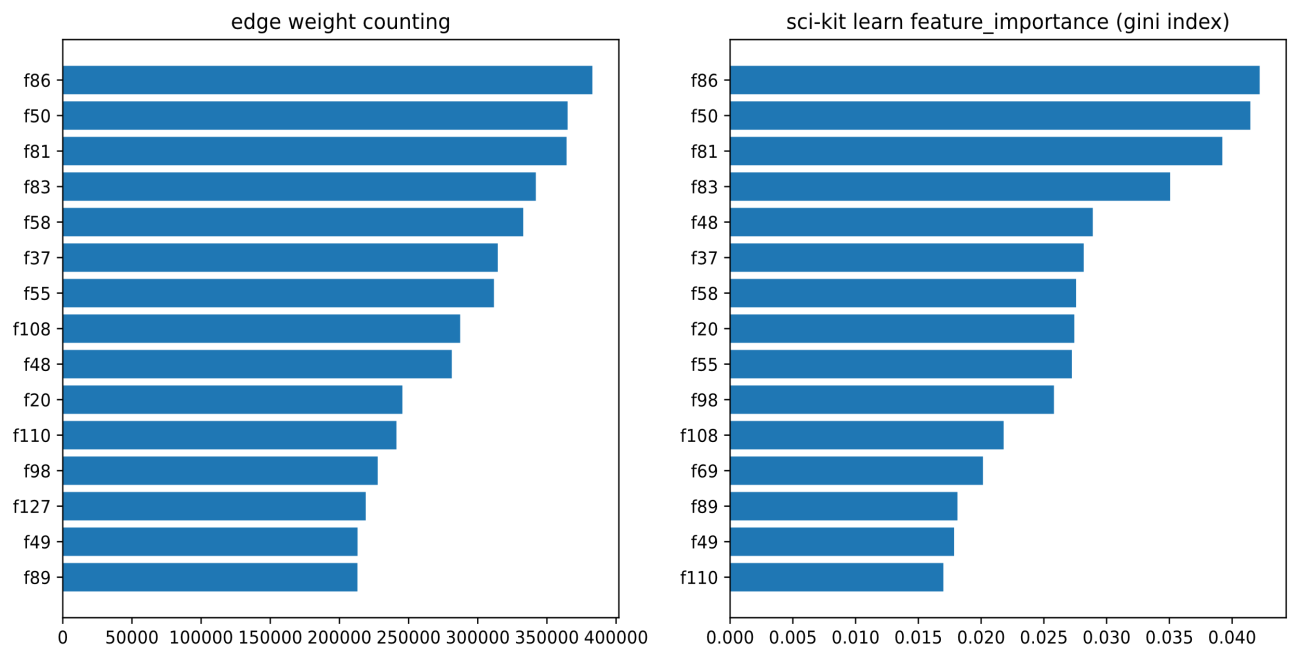
\includegraphics[width=0.95\columnwidth]{figures/network_top_feature.png}
	\caption{Az RFC legfontosabb jellemzői. Bal oldalon az általam írt algoritmus eredménye, jobb oldalon a sci-kit learn függvényével kapott eredmény.}
	\label{fig:myfimp}
\end{figure}

Feltételezésem az volt, hogy a gráf struktúrájából adódóan meg tudok határozni a modell számára szignifikáns jellemzőket amelyeket, ha eltávolítunk az adathalmazból, a modell pontossága jelentősen romlani fog. Egy jellemző fontosságát úgy határoztam meg, hogy a súlyozott gráf jellemzőhöz tartozó csomópontjának vettem a fokszámát (csomóponthoz tartozó élek súlyainak összegét). A fokszámokat ki tudtam számolni a szomszédossági mátrix alapján. A kapott eredményeket csökkenő sorrendbe rendeztem, és összehasonlítottam a Sci-kit learn feature\_importance módszerével kapott eredménnyel. A két módszerrel nagyon hasonló eredményt kaptam, amit láthatunk a \ref{fig:myfimp}. ábrán. 

Miután a modell számára legfontosabb jellemzőket meghatároztam, megnéztem hogyan változik a RFC pontossága, ha eltávolítom a legfontosabb feature-öket. Mit láthatjuk a \ref{fig:retrain_agane}. ábrán, a modell pontossága nem romlik jelentően még akkor sem, ha feature-ök több mint felét eltávolítottuk.

\begin{figure}[ht]
	\centering
	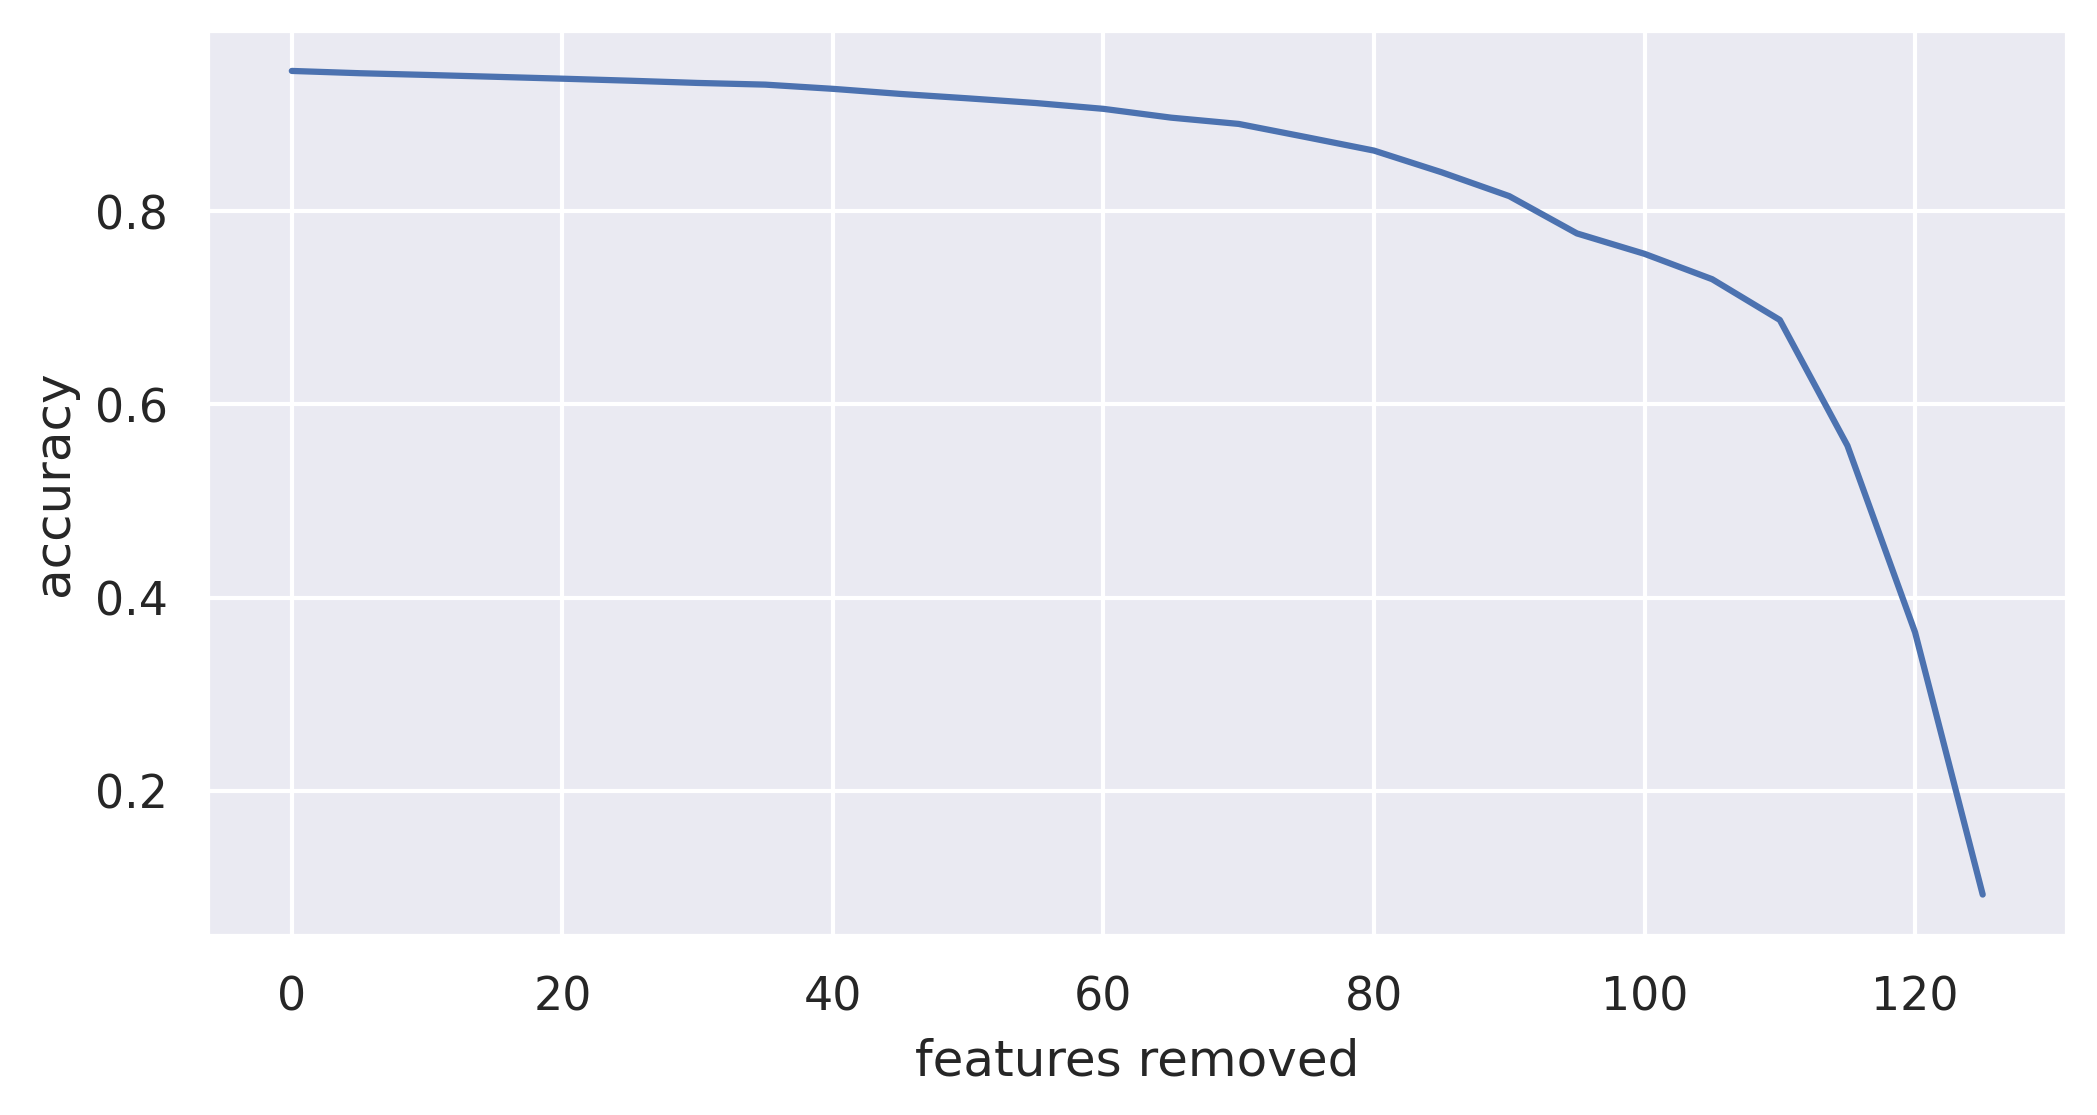
\includegraphics[width=0.8\columnwidth]{figures/network_race_graph.png}
	\caption{A rassz predikciós modell pontosságának kirajzolása az eltávolított jellemzők számától függően.}
	\label{fig:retrain_agane}
\end{figure}
